\documentclass{beamer}
\usepackage{amsmath}

\usetheme{PaloAlto}

\title[Dynamics and Flows]{Dynamics and Flows}
\author[Aadhithya Saravanan]{Aadhithya Saravanan\\[0.5em] Mentor: Aprameya Girish Hebbar}
\date{May 5, 2026}

\begin{document}

\section{Introduction}

\begin{frame}
    \titlepage
\end{frame}

\begin{frame}{Introduction}
    We will begin with one of the simplest differential equations,
    \[
        \frac{dx}{dt} = ax
    \]
    where $a$ is a constant. Here, $x=x(t)$ is a function that we are solving for, where its derivative with respect to $t$ is given by the right-hand side. This equation models exponential growth or decay, depending on the sign of $a$. The solution to this equation is given by
    \[
        x(t) = x(0)e^{at}
    \]
    where $x(0)$ is the initial condition. This simple model can be used to describe a wide range of phenomena, from population growth to radioactive decay.
\end{frame}

\begin{frame}{Introduction}
    To solve this equation, we can use the method of separation of variables. We can rewrite the equation as
    \[
        \frac{1}{x} dx = a dt
    \]
    Integrating both sides, we get
    \[
        \ln|x| = at + C
    \]
    where $C$ is the constant of integration. Exponentiating both sides, we obtain
    \[
        |x| = e^{at + C} = e^C e^{at}
    \]
    Letting $x(0) = e^C$, we can write the solution as
    \[
        x(t) = x(0)e^{at}
    \]
\end{frame}

\begin{frame}{Introduction}
    More importantly than the solution to this specific equation, we want to know if the solution we have found is unique. Let $u(t)$ be another solution to the same equation with the same initial condition. Then we have
    \[
        \frac{du}{dt} = au
    \]
    We can take the derivative of $u(t)e^{-at}$ with respect to $t$:
    \[
        \frac{d}{dt}[u(t)e^{-at}] = \frac{du}{dt}e^{-at} - ae^{-at}u(t) = (au - au)e^{-at} = 0
    \]
\end{frame}

\begin{frame}{Introduction}
    Since the derivative is zero, $u(t)e^{-at}$ is a constant, say $C$. Therefore,
    \[
        u(t) = Ce^{at}
    \]
    Using the initial condition $u(0) = x(0)$, we get $C = x(0)$, so
    \[
        u(t) = x(0)e^{at} = x(t)
    \]
    This shows that the solution is unique. However, this is just a specific example. In general, we need to establish conditions under which solutions to differential equations exist and are unique. This is where the Existence and Uniqueness Theorem comes into play, which will be discussed after we cover some more examples and concepts in the next sections.
\end{frame}

\section{Systems of Differential Equations}

\begin{frame}{Systems of Differential Equations}
    A system of differential equations is a collection of $n$ differential equations of the form
    \[x_1' = f_1(t, x_1, x_2, \ldots, x_n)\]
    \[x_2' = f_2(t, x_1, x_2, \ldots, x_n)\]
    \[\vdots\]
    \[x_n' = f_n(t, x_1, x_2, \ldots, x_n)\]
    Each $f_j$ is a real-valued function of the $n+1$ variables $t, x_1, x_2, \ldots, x_n$. We can write this system in vector form as
    \[
        X=
        \begin{pmatrix}
            x_1 \\
            x_2 \\
            \vdots \\
            x_n
        \end{pmatrix}
    \]
\end{frame}

\begin{frame}{Systems of Differential Equations}
    Then, the system can be expressed as
    \[
        X' = F(t, X)
    \]
    where
    \[F(t, X)=
    \begin{pmatrix}
        f_1(t, x_1, x_2, \ldots, x_n) \\
        f_2(t, x_1, x_2, \ldots, x_n) \\
        \vdots \\
        f_n(t, x_1, x_2, \ldots, x_n)
    \end{pmatrix}
    \]
    A solution of this system is then a function of the form
    \[X(t)=(x_1(t), x_2(t), \ldots, x_n(t))\]
    such that $X'(t) = F(t, X(t))$.
\end{frame}

\begin{frame}{Systems of Differential Equations}
    Let us look at a specific example of a system of differential equations. Consider the following system:
    \[x'=y\]
    \[y'=-x\]
    We let $x_1=x$ and $x_2=y$, so we can write this system in vector form as
    \[X'=
    \begin{pmatrix}
        x' \\
        y'
    \end{pmatrix}=
    \begin{pmatrix}
        0 & 1 \\
        -1 & 0
    \end{pmatrix}
    \begin{pmatrix}
        x \\
        y
    \end{pmatrix}
    \]
\end{frame}

\begin{frame}{Systems of Differential Equations}
    The curve $X(t)=(a\cos t, a\sin t)$ for any $a\in \mathbb{R}$ is a solution to this system, since
    \[x'(t)=-a\sin t=y(t)\]
    \[y'(t)=a\cos t=-x(t)\]
    We can look at the slope field of this system along with a few solution curves to get a better understanding of the behavior of the system.
\end{frame}

\begin{frame}{Systems of Differential Equations}
    \begin{block}{Slope Field and Solution Curves}
        \begin{center}
        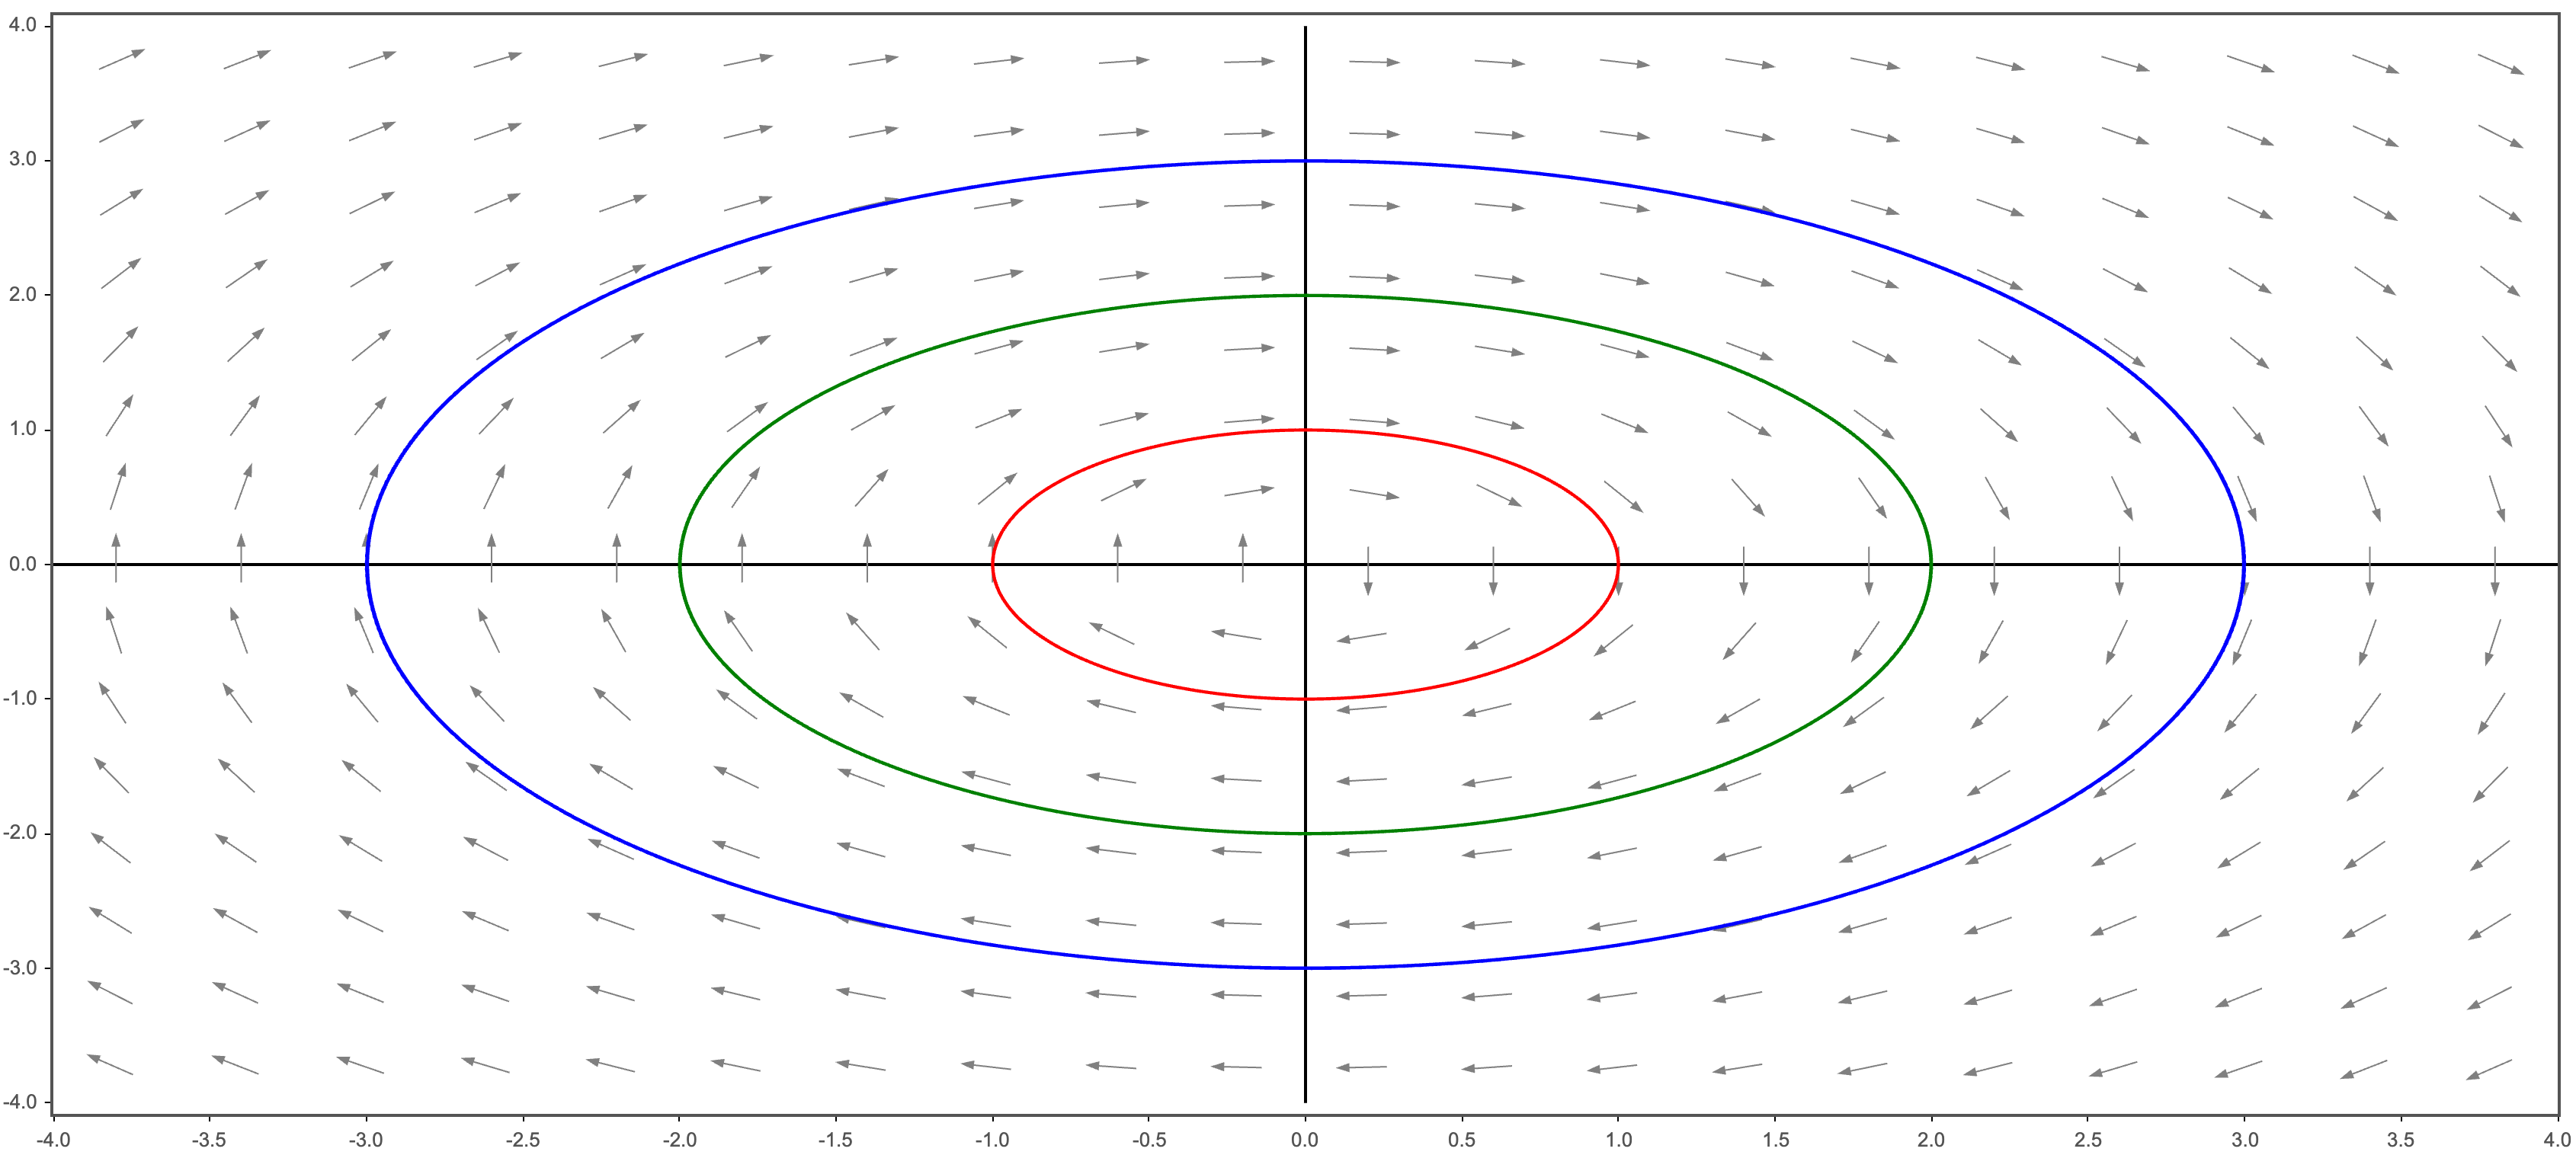
\includegraphics[width=0.9\textwidth]{PlanarSystem.png}
    \end{center}
    \end{block}
    As we can see from the slope field, the solution curves are circles centered at the origin. The system describes a simple harmonic oscillator, where the solutions represent periodic motion.
\end{frame}

\section{Section 4}

\begin{frame}{Section 4}
\end{frame}

\begin{frame}{Section 4}
\end{frame}

\end{document}